\section{Experimental Setup}
As was discussed in \S\ref{sec:benchmark-datasets}, there are many issues with the benchmarks that were proposed by \cite{yuan_explainability_2021}. Therefore, a major goal of this work was to confirm the intuition that these benchmarks were off. Then, the aim was to create a new set of benchmarks against which GNN interpretation models can be tested against. In this section, the methodology of these experiments will be walked through.

\subsection{Validation of Incorrectness in Benchmark Datasets}
As was shown in figure \ref{fig:tree-cycles-proposed-gt}, the proposed ground truth for the tree cycles dataset that was introduced by GNNExplainer is supposed to be the graph motifs that are encoded as the node classes. Specifically, for a node that is in a cycle, the proposed groundtruth is all of the edges in the size six cycle. Similarly, for a node that is in the tree portion of the dataset, the supposed groundtruth is all the edges in the tree. 

To validate our intuition that this was not what the GNN was necessarily learning, we conducted the following experiment:
\begin{enumerate}
	\item We trained a GNN on the tree-cycles dataset and ensured it had good validation accuracy \~95\%. Since the nodes have no node features, it is clear that the GNN is \textit{only} learning from the computational graph that it is given.
	\item For a few sample nodes classified as cycle nodes, we collected every connected size six subgraph.
	\item These subgraphs were fed to the GNN and were ranked according to the mutual information of the outputed classification distribution.
	\item These samples were then plotted to compare them against the proposed ground truth.
\end{enumerate}
While not a comprehensive review, the computational resources needed to check every node were prohibitive. Note that this metric for choosing the best subgraph comes directly from the GNNExplainer paper meaning that if their assumption was valid, the entire cycle would be chosen as the ground truth. The nodes chosen for this experiment were nodes 557, 566, and 511. In figure \ref{fig:tree-cycles-gt} are the resulting, subgraphs of size 6.
\begin{figure}[H]
	\centering
	\begin{subfigure}{0.49\textwidth}
		\centering
		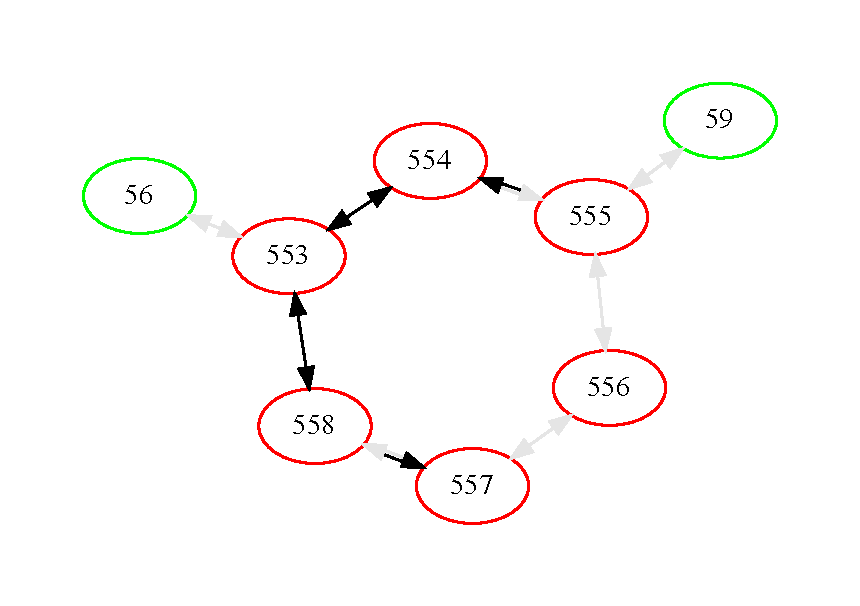
\includegraphics[width=0.95\linewidth]{images/tree-cycles-557.pdf}
	\end{subfigure}
	\begin{subfigure}{0.49\textwidth}
		\centering
		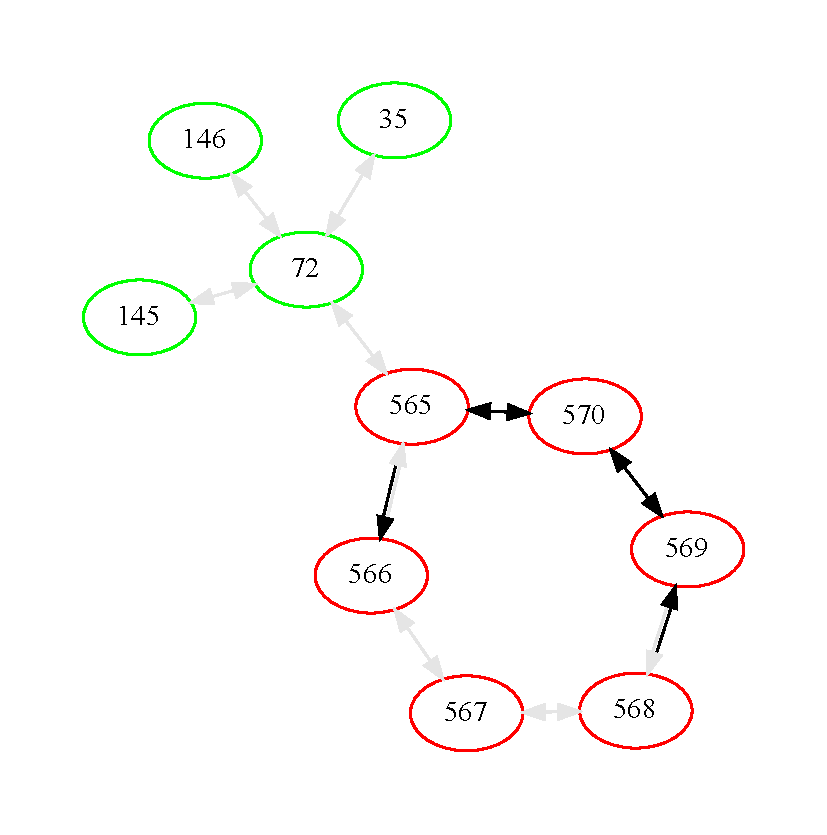
\includegraphics[width=0.95\linewidth]{images/tree-cycles-566.pdf}
	\end{subfigure}
	\begin{subfigure}{0.49\textwidth}
		\centering
		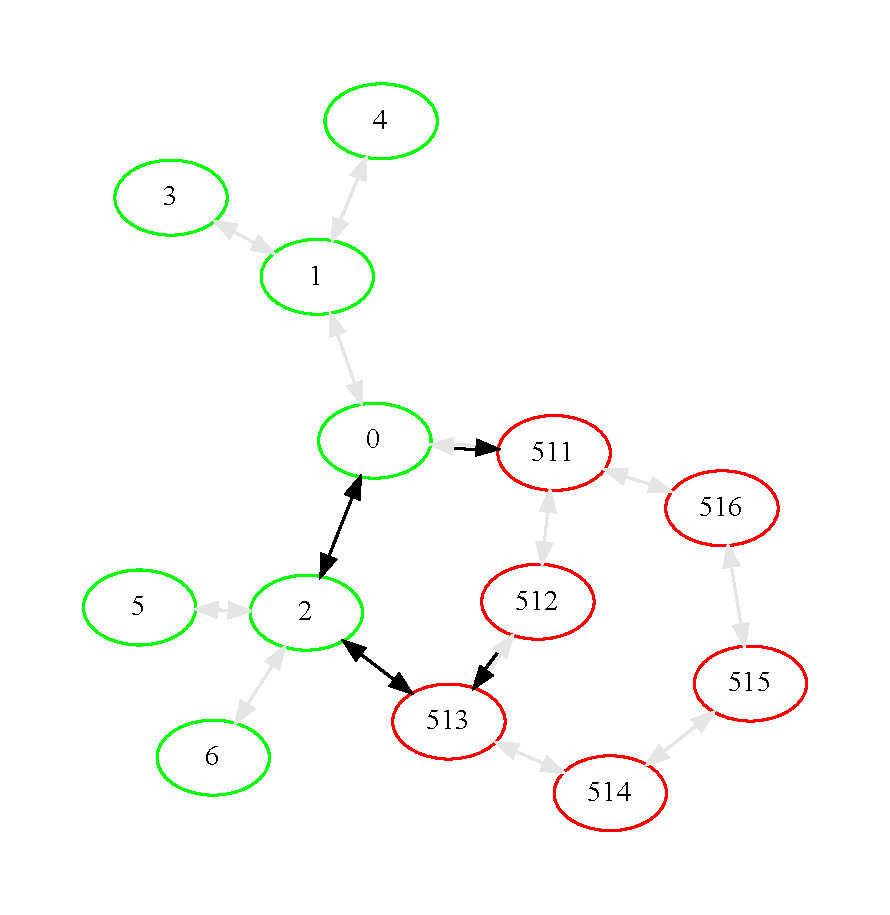
\includegraphics[width=0.95\linewidth]{images/tree-cycles-511.pdf}
	\end{subfigure}
	\caption{Found best subgraphs of size six for nodes 557, 566, and 511}
	\label{fig:tree-cycles-gt}
\end{figure}

Indeed, in none of the examples did a full ring structure get predicted. For nodes 557 and 566 it is clear that the most important subgraph uses about half the ring and has feedback structures inside of it with edges going both ways on intermediate nodes. In node 511, the interpretation barely comes from the ring structure and the GNN passes information through the edges of the tree structures. Clearly, it is not obvious that the motifs that the graph was defined on are not the groundtruth. Furthermore, the groundturth is \textit{highly} dependent on the GNN that is trained. With regards to the tree-cycle dataset, there are many different GNNs that peform equally well but have different groundtruths. Hence, it is difficult to use this dataset for GNN interpretation validation. While one could train GNNs until the motifs do become the correct groundtruth, it is hard to validate that any training run has achieved this goal.



\subsection{Noise Filtering Experiment}

\subsection{Tree Embedding Experiment}

\newpage
